\chapter{METODOLOGI PENELITIAN}
Pada bagian ini peniliti menggunakan dua jenis data yaitu data primer dan data sekunder. Data primer adalah data yang diperoleh dari hasil kuisoner dan data sekunder yang diperoleh dari hasil penilitian sebelumnya.

\section{Data dan Pengumpulan Data}
Penulis menggunakan beberapa tahap atau metode dalam melakukan penilitian untuk menyusul proposal skripsi, yaitu :

\begin{enumerate}
    \item Studi Pustaka \\ Peneliti mengumpulkan data dengan cara mencari dari internet dan jurnal yang menyangkut atau jurnal yang membahas photon unity networking dalam pembuatan game multiplayer.
    \item Observasi \\ Peniliti mengumpulkan data dengan cara memainkan sekaligus mengamati secara langsung permainan sejenis yang sudah ada.
\end{enumerate}

\section{Rancangan Sistem(software/hardware)}
    Pada penilitian ini membutuhkan \textit{software} dan perangkat keras untuk melakukan pembuatan game first person shooter. Berikut ini spesifikasi rancangan sistem penilitian yang dijabarkan pada Tabel 3.1
    
    \begin{table}[h]
        \centering
        \begin{tabular}{|ll|lll}
        \cline{1-2}
        \multicolumn{2}{|c|}{Software}                                                &  &  &  \\ \cline{1-2}
        \multicolumn{1}{|l|}{Sistem Operasi} & Windows 11                             &  &  &  \\ \cline{1-2}
        \multicolumn{1}{|l|}{Tools}          & Unity                                  &  &  &  \\ \cline{1-2}
        \multicolumn{2}{|c|}{Perangkat Keras}                                         &  &  &  \\ \cline{1-2}
        \multicolumn{1}{|l|}{Processor}      & Amd Ryzen 5 5400H With Radeon Graphics &  &  &  \\ \cline{1-2}
        \multicolumn{1}{|l|}{Memory}         & 8192MB Ram                             &  &  &  \\ \cline{1-2}
        \multicolumn{1}{|l|}{Video Card}     & Nvidia GeForce RTX 3050                &  &  &  \\ \cline{1-2}
        \multicolumn{1}{|l|}{SSD}            & 460GB                                  &  &  &  \\ \cline{1-2}
        \end{tabular}
        \end{table}
\subsection{Rancangan Algoritma Matchmaking}
Matchmaking dalam fitur permainan ini berperan sangat penting dan merupakan peran utama. Dalam peran tersebut, matchmaking mempertemukan antar pemain yang sedang aktif dalam melakukan pencarian room. Berikut penjelasan algoritma dalam bentuk \textit{flowchart} pada gambar 1.
\begin{figure}[h]
    \centering
    \caption{uhy}
    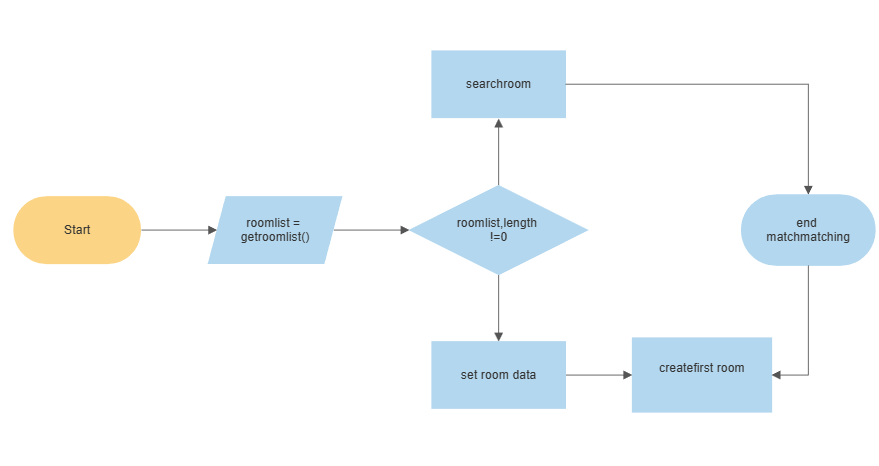
\includegraphics[width=15cm]{flowchart-matchmaking}
    \label{tb:uhuy}
    \end{figure}
\section{Metode dan Variabel Penelitian}
Pada bagian ini diuraikan pembuatan/implementasi sistem,   metode/algoritma yang digunakan, jika memungkinkan disertai dengan flowchart dari proses implementasi dan algoritma yang digunakan.

\section{Teknik Pengujian}
Pada bagian ini diuraikan tentang keterkaitan antarfaktor dari data yang diperoleh  berdasarkan masalah yang dirumuskan pada bagian rumusan masalah. Selanjutnya,  masalah tersebut diselesaikan dengan metode/algoritma yang digunakan, dianalisis proses dan hasil penyelesaian masalah tersebut.  Dalam hal ini, perlu disebutkan parameter-parameter yang akan diuji dan dianalisis pada penelitian yang dimaksud beserta dengan alat ujinya.

\section{Hasil yang diharapkan}
Pada bagian ini dicantumkan prediksi hasil penelitian. Dalam hal ini, dapat dipaparkan kira-kira hasil akhir penelitian yang akan dicapai berupa apa?